% Here we include more details on all aspects in Section 2 if they can be useful for the development team.

\subsection{External Interface Requirements}

\subsubsection{User Interfaces}


Below are some sample screenshots from the project's user interfaces with Samsung Galaxy S9 viewport: \\
\begin{figure}[H]
    \centering
    \begin{minipage}{0.45\textwidth}
        \centering
        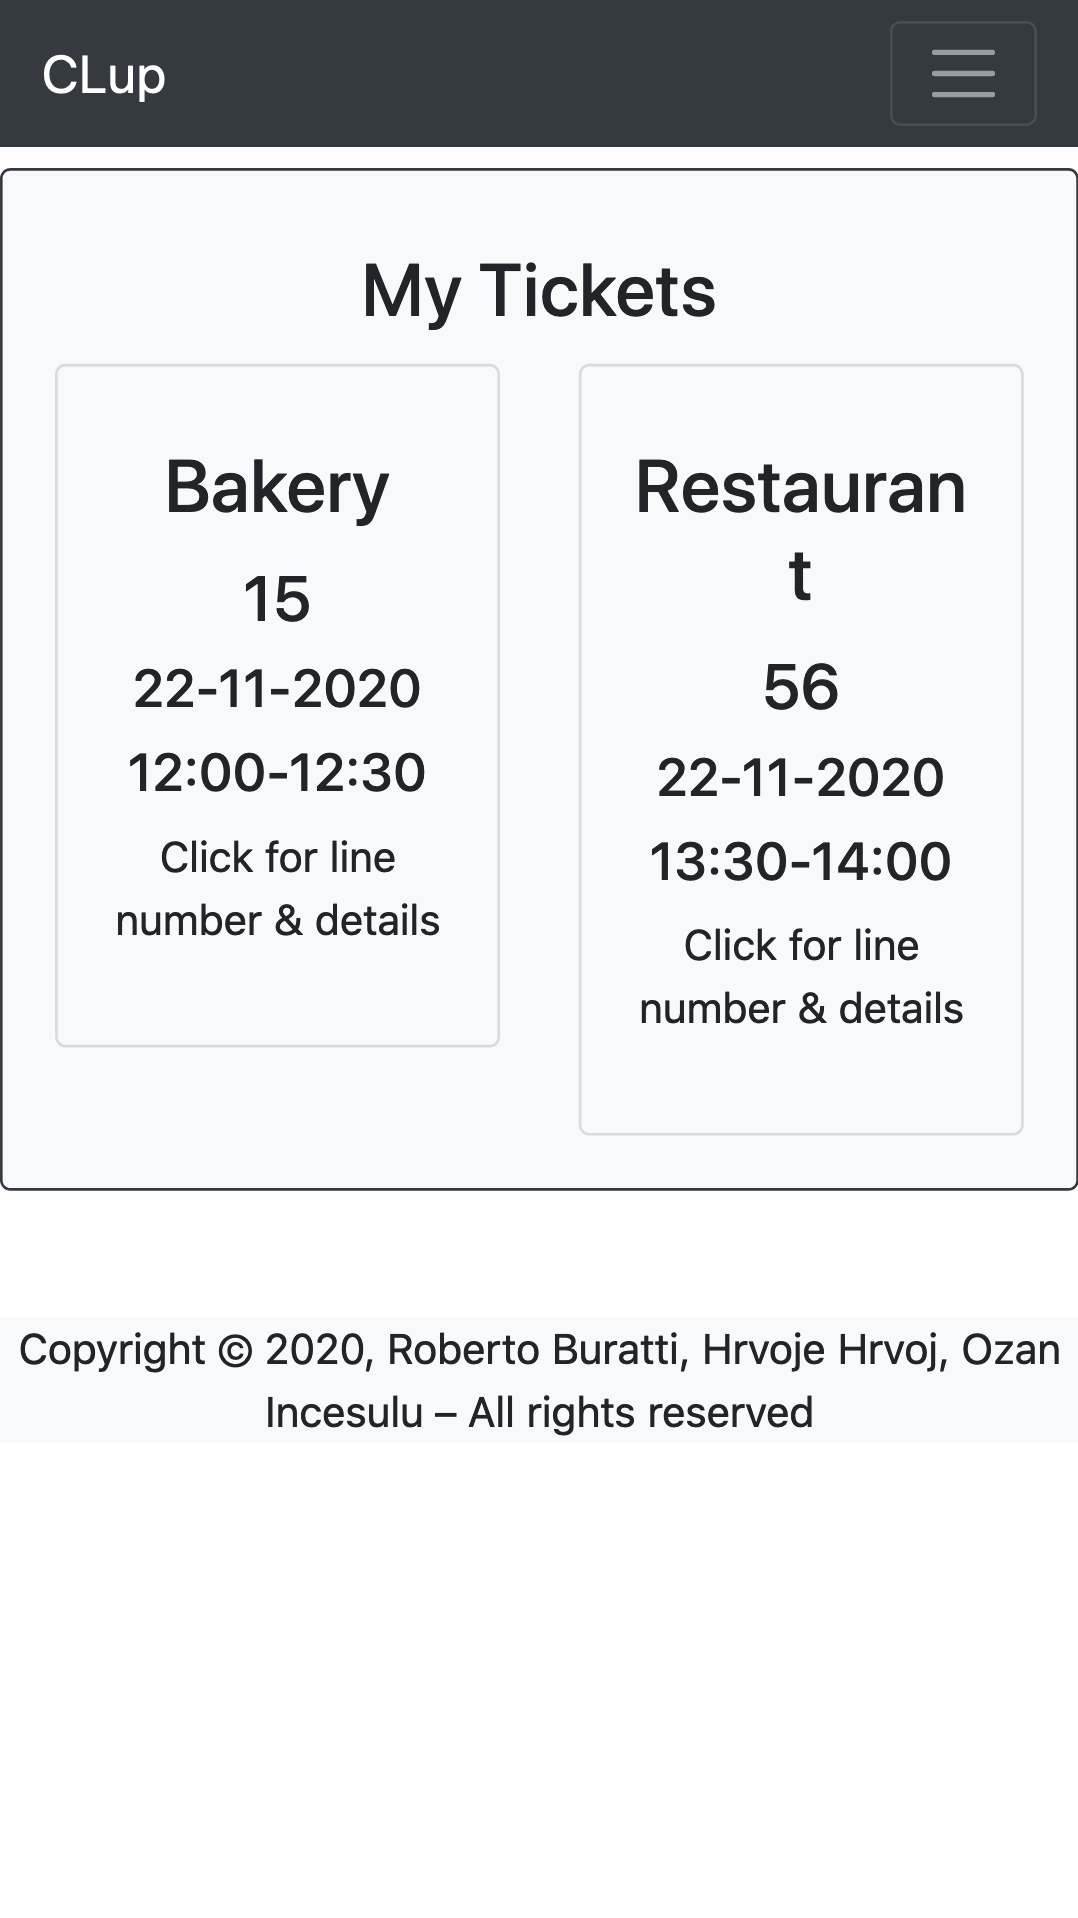
\includegraphics[width=0.9\textwidth]{Images/Screenshots/ticketList.png}
        \caption{Screenshot: List tickets}
    \end{minipage}\hfill
    \begin{minipage}{0.45\textwidth}
        \centering
        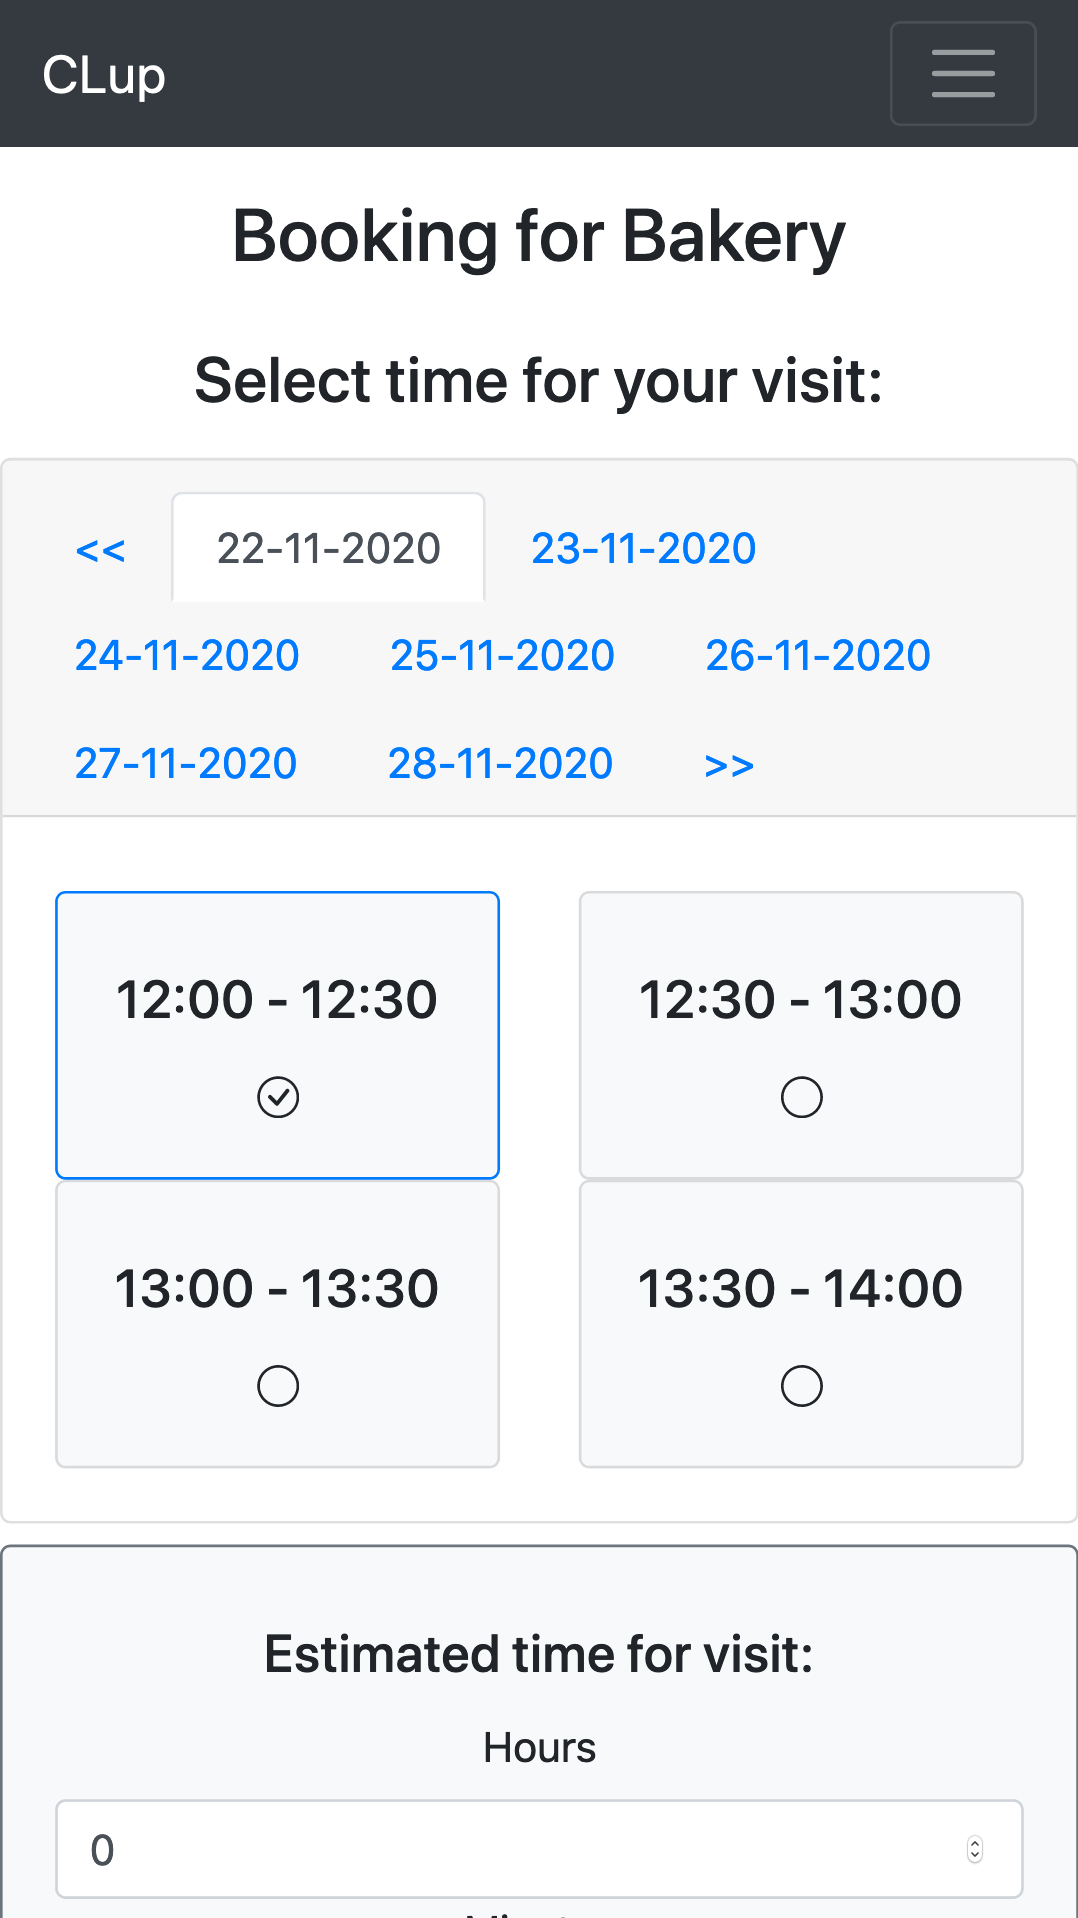
\includegraphics[width=0.9\textwidth]{Images/Screenshots/booking.png} % second figure itself
        \caption{Screenshot: Booking a new ticket}
    \end{minipage}
\end{figure}

\begin{figure}[H]
    \centering
    \begin{minipage}{0.45\textwidth}
        \centering
        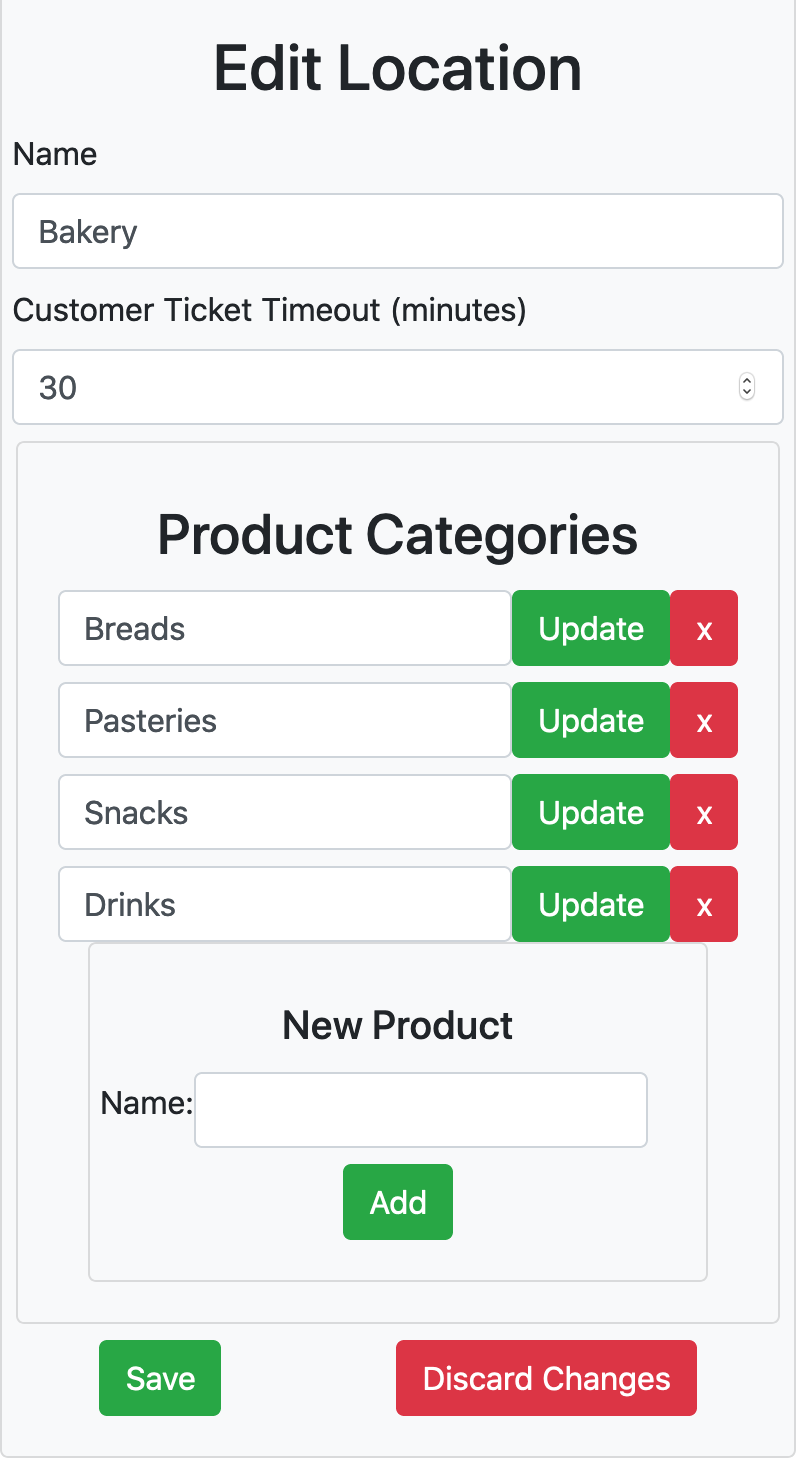
\includegraphics[width=0.9\textwidth]{Images/Screenshots/editLocation.png}
        \caption{Screenshot: Edit location screen of manager}
    \end{minipage}\hfill
    \begin{minipage}{0.45\textwidth}
        \centering
        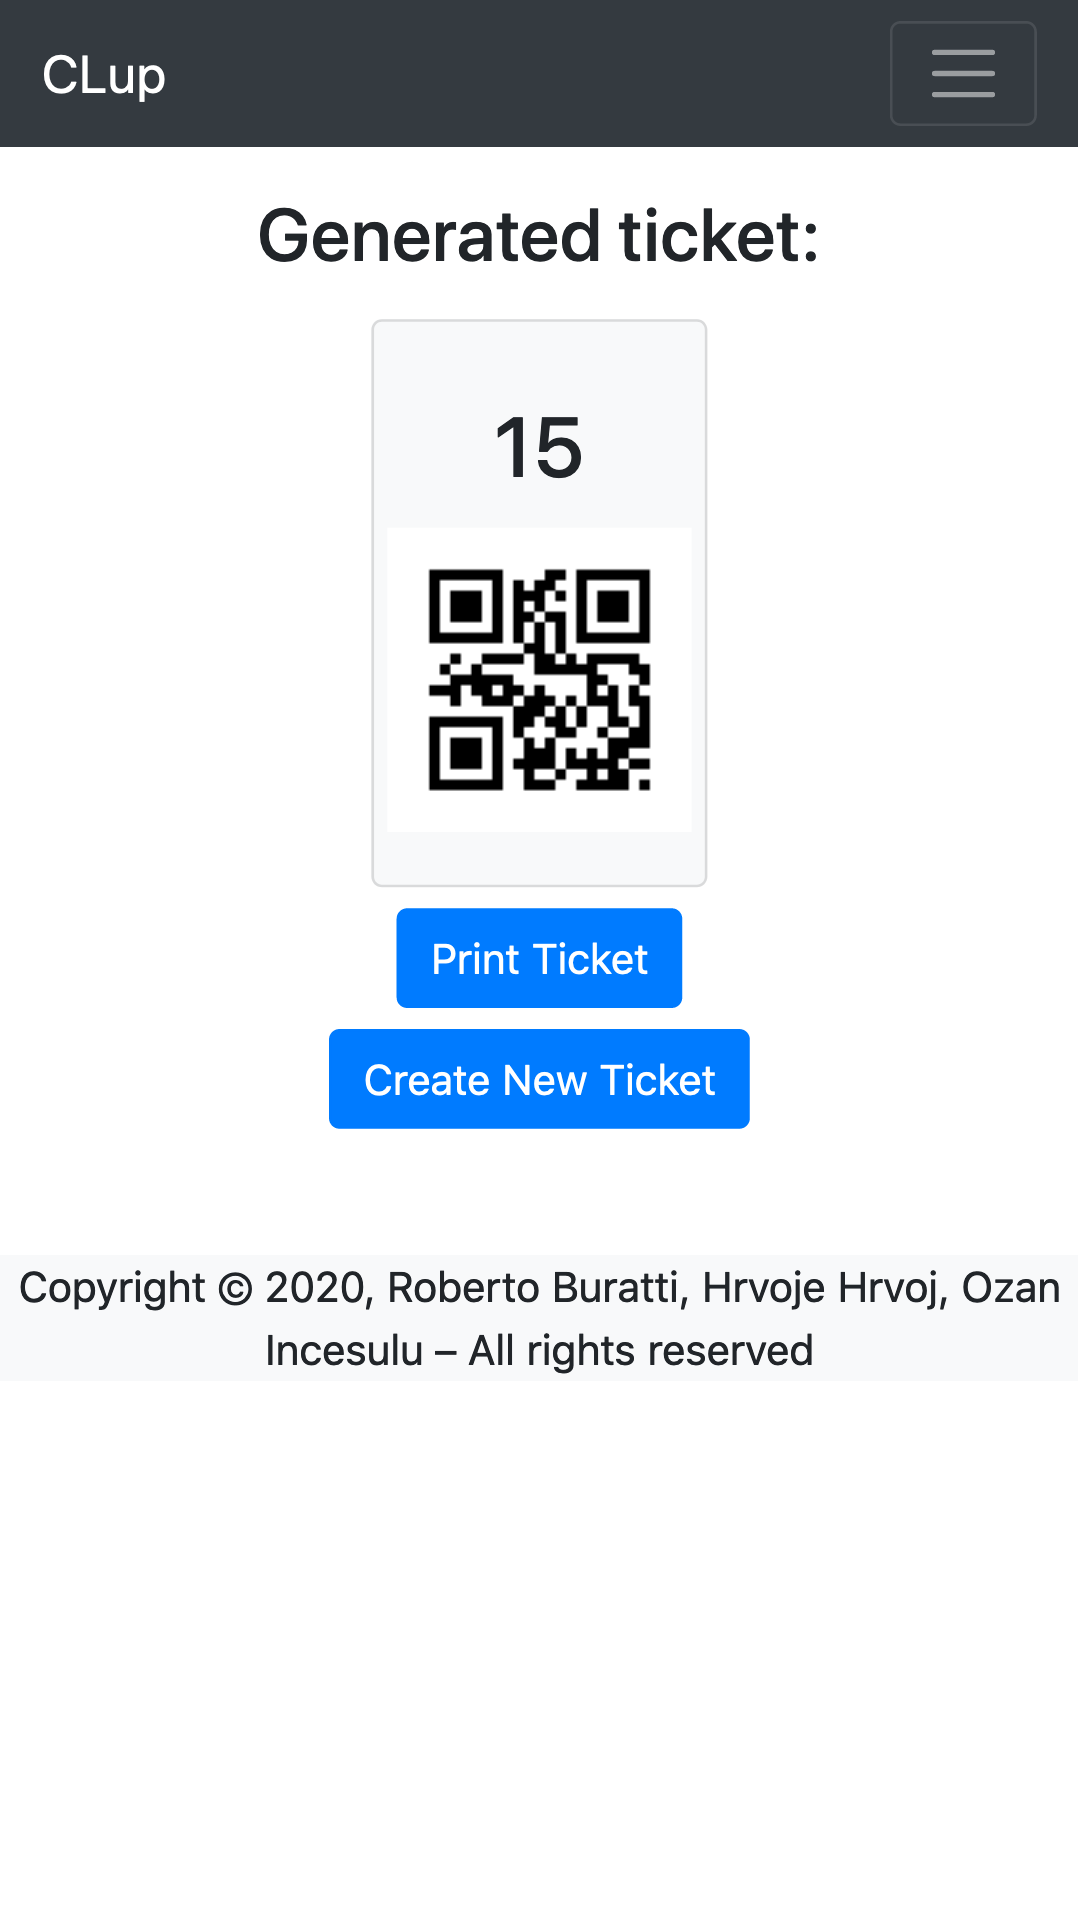
\includegraphics[width=0.9\textwidth]{Images/Screenshots/ticketGenerate.png} % second figure itself
        \caption{Screenshot: Ticket generate screen of clerk}
    \end{minipage}
\end{figure}

\begin{figure}[H]
    \centering
    \begin{minipage}{0.45\textwidth}
        \centering
        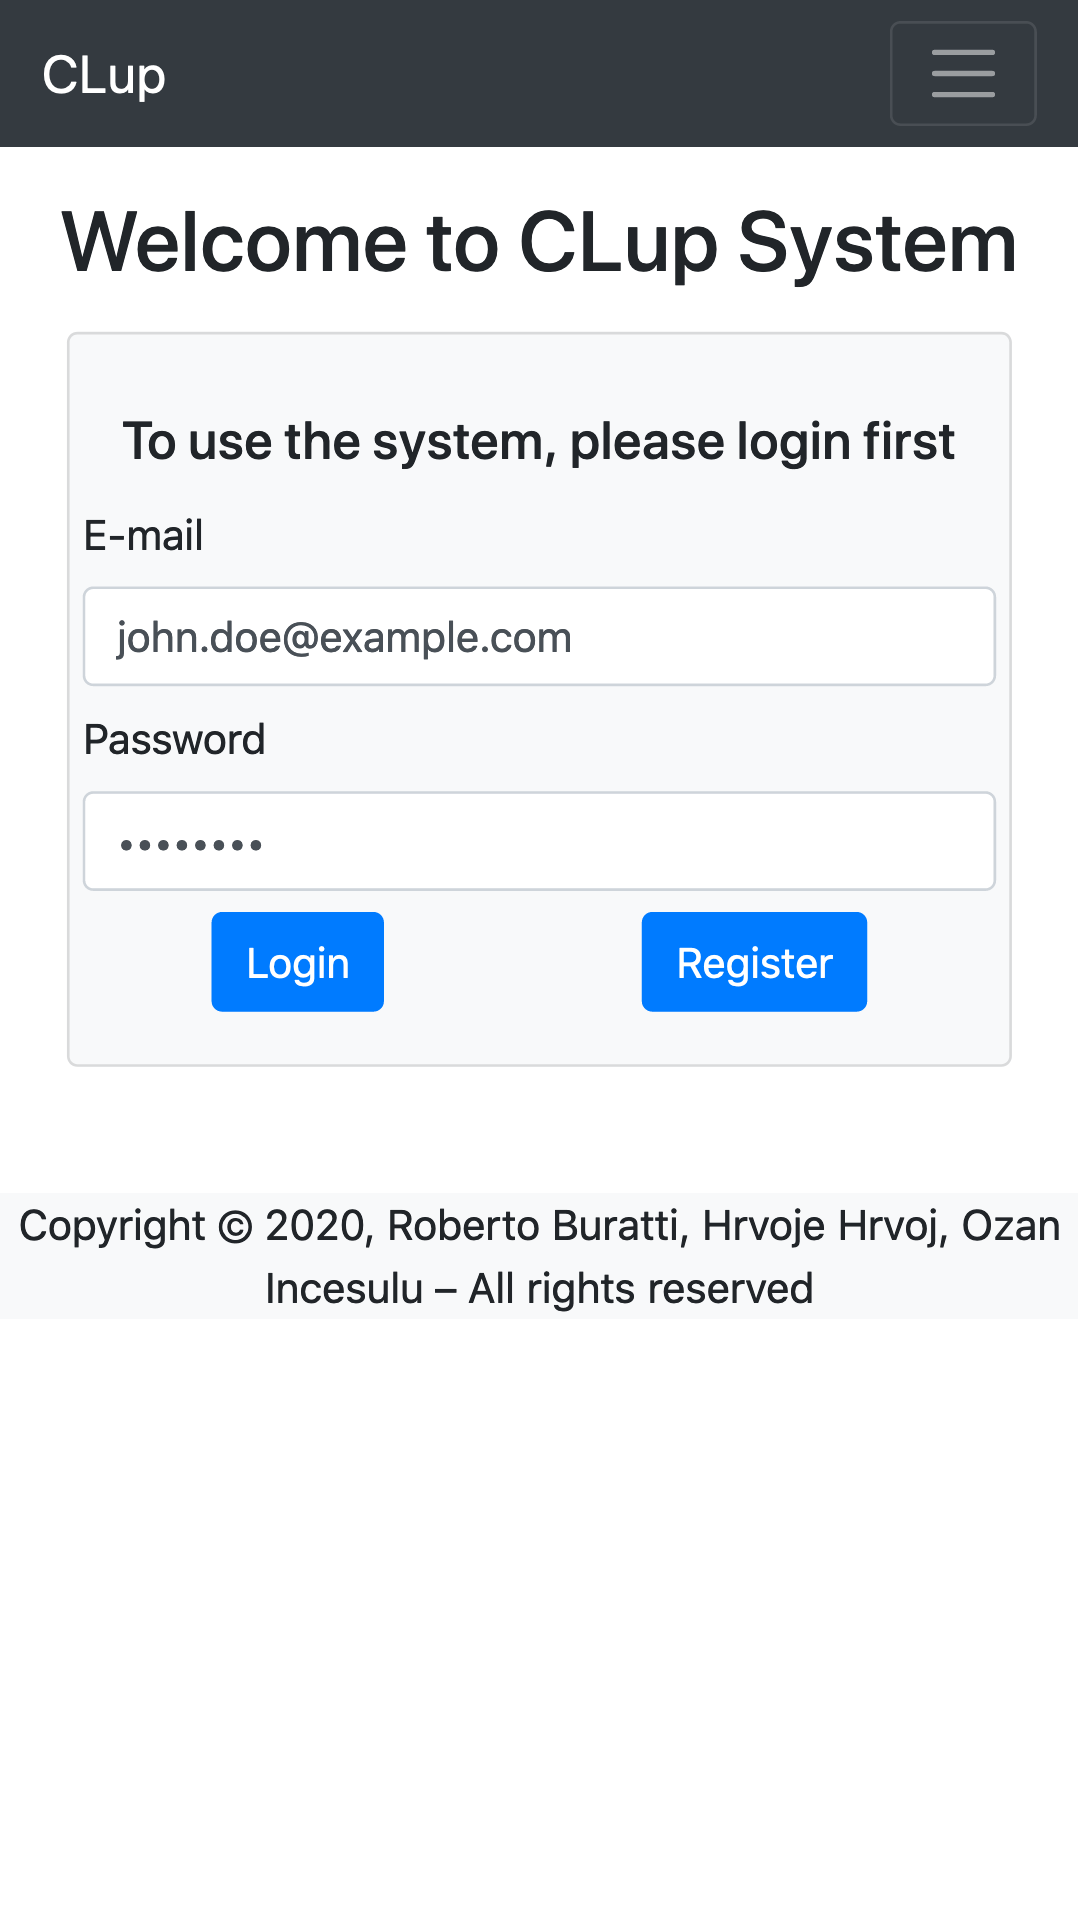
\includegraphics[width=0.9\textwidth]{Images/Screenshots/login.png}
        \caption{Screenshot: Login screen}
    \end{minipage}\hfill
    \begin{minipage}{0.45\textwidth}
        \centering
        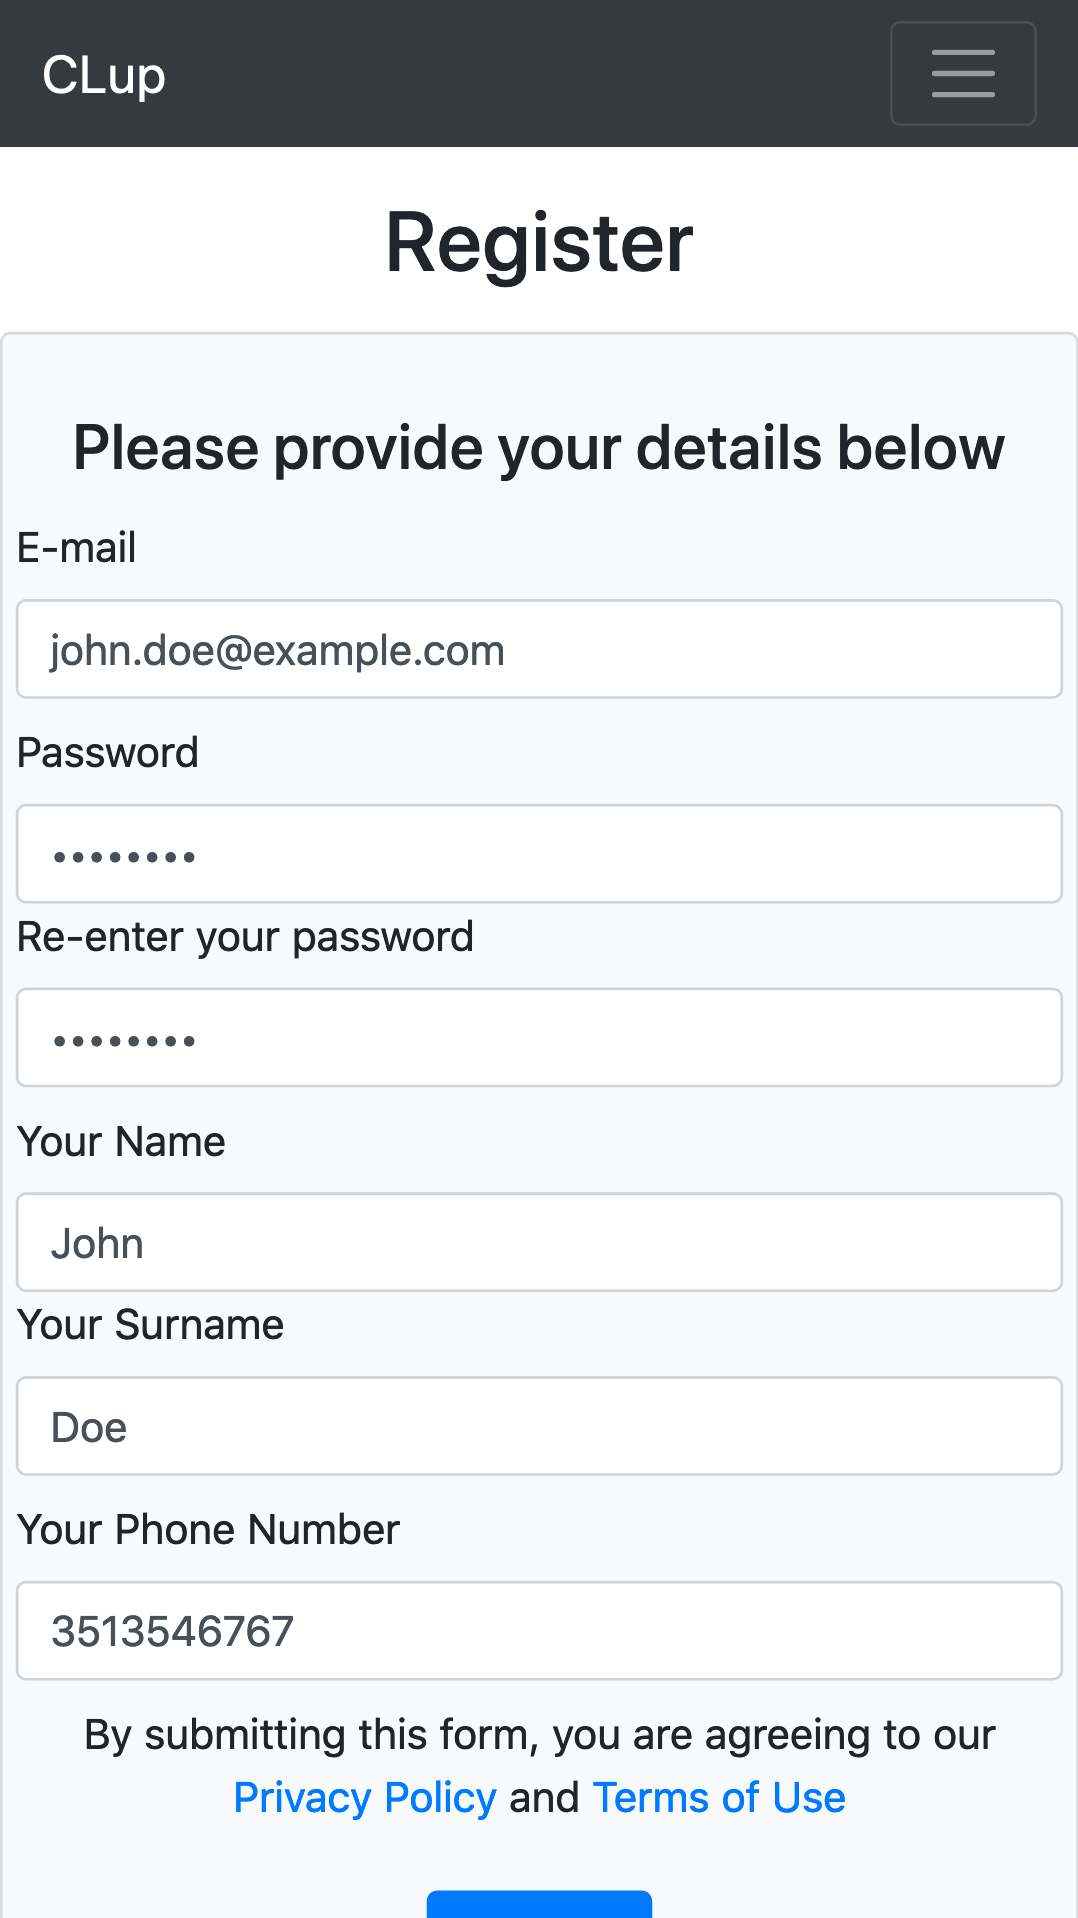
\includegraphics[width=0.9\textwidth]{Images/Screenshots/register.png} % second figure itself
        \caption{Screenshot: Register screen}
    \end{minipage}
\end{figure}
% Actual mockups of user interfaces

\subsubsection{Hardware Interfaces}
% TODO: @Hrvoje These 3
% Do we integrate with external hardware?

%Specify the logical characteristics of each interface between the software product and the hardware elements of the system.
%This includes configuration characteristics (number of ports, instruction sets, etc.).
%It also covers such matters as what devices are to be supported, how they are to be supported, and protocols.
%For example, terminal support may specify full-screen support as opposed to line-by-line support.

The application will be able to run on desktop as well as tablet and smartphone. Operating system or exact performances of the device you are using are not important since the vast majority of devices will be supported. On the user end it would be best if users could use a smartphone or a tablet so they could bring it with them to the store. Clerk should have a smartphone as mention in the domain assumptions with a working camera module. The manager should mainly use a desktop computer so he could manage store information easily, he should be able to do all his tasks from smartphone or a tablet but a desktop computer remains recommended.

\subsubsection{Software Interfaces}
% Do we integrate with custom software, expose an API?

%Specify the use of other required software products (e.g., a data management system, an operating system, or a mathematical package), and interfaces with other application systems (e.g., the linkage between an accounts receivable system and a general ledger system).
%For each required software product, specify:
%a) Name;
%b) Mnemonic;
%c) Specification number;
%d) Version number;
%e) Source.

Application should run on every operating system such as Windows, Linux or MacOS for desktop device, and Android or iOS for mobile devices. Application will use QR code generator to produce QR code which will be scanned when entering the store and which will contain all the information related to the visit time of the customer.

\subsubsection{Communication Interfaces}
% What is a communication interface? the Internet? RF port? Radio? Bluetooth?

%Specify the various interfaces to communications such as local network protocols.
Device should have an active internet connection and the application should communicate through TCP/IP.

\subsection{Functional Requirements}
% Use draw.io, compatible with GitHub.

% Definition  of  use  case  diagrams,  use  cases  and  associated sequence/activity diagrams, and mapping on requirements

% Use case diagram

% For each use case:
%   Use case table
%   Use case sequence diagram
\subsubsection{Customer}

\begin{figure}[H]
    \centering
    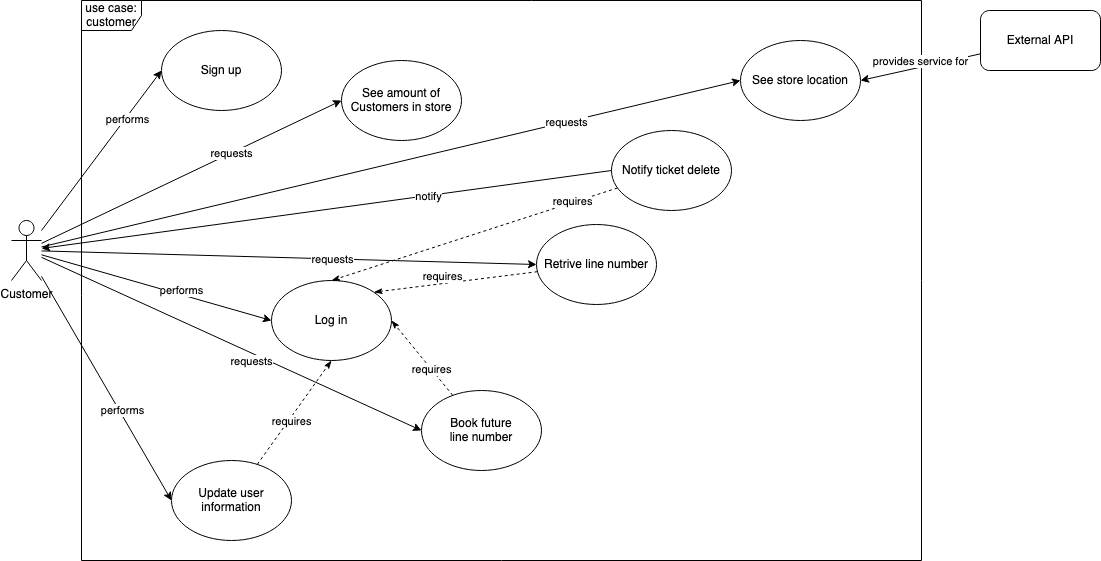
\includegraphics[height=0.5\textwidth]{Images/UseCaseDiagrams/Customer.png}
    \caption{Use Case Diagram for Customer}
\end{figure}
\textbf{Use cases}
\begin{table}[H]
    \begin{tabular}{|p{8cm}|p{8cm}|}
        \hline
        \textit{Name}    & \textbf{Book future line number} \\ \hline
        \textit{Actors} & Customer \\ \hline
        \textit{Entry conditions} & The customer is logged in the application and wants to book a visit to the store. \\ \hline
        \textit{Event flows}      & \tabitem The customer clicks on the "Book a Visit" button in the application. \\
        & \tabitem The application asks the time slot and the estimated time of the visit presenting as default value the average of the previous times of visit of the same user. \\
        & \tabitem The customer sets the time slot and the estimated time of their visit. \\
        & \tabitem The application asks what category of products the customer wants to buy. \\
        & \tabitem The customer set the products categories. \\
        & \tabitem The application requests the line number from the server. \\
        & \tabitem The application generates the QR code on the response from the server. \\
        \hline
        \textit{Exit conditions} & The customer has booked a visit for the store. \\ \hline
        \textit{Exceptions} & \tabitem The server cannot retrieve the line number since the time slot is full.\\ \hline
    \end{tabular}
    \caption{Use Case: Book future line number}
\end{table}
\begin{figure}[H]
    \centering
    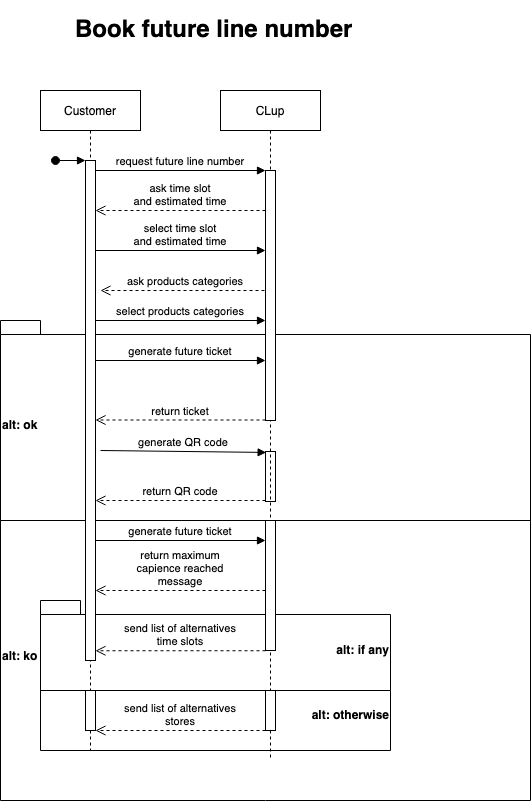
\includegraphics[height=0.5\textwidth]{Images/SequenceDiagrams/Customer/BookFutureLineNumberUseCaseSequenceDiagram.png}
    \caption{Sequence Diagram for Use Case: Book future line number}
\end{figure}
\begin{table}[H]
    \begin{tabular}{|p{8cm}|p{8cm}|}
        \hline
        \textit{Name}    & \textbf{See amount of customers in the store} \\ \hline
        \textit{Actors} & Customer \\ \hline
        \textit{Entry conditions} & The customer is logged in the application and wants to know how many customers are in the store in order to decide whether to book a visit or retrieve a line number \\ \hline
        \textit{Event flows}      & \tabitem The customer clicks on the  "Live Store Info" button. \\
        & \tabitem The application sends a count request to the server. \\
        & \tabitem The server returns the live data for the amount of customers in the store for each time slot. \\
        \hline
        \textit{Exit conditions} & The customer knows the amount of customers in the store and can plan their visit. \\ \hline
        \textit{Exceptions} & \\ \hline
    \end{tabular}
    \caption{Use Case: See amount of customers in the store}
\end{table}

\begin{figure}[H]
    \centering
    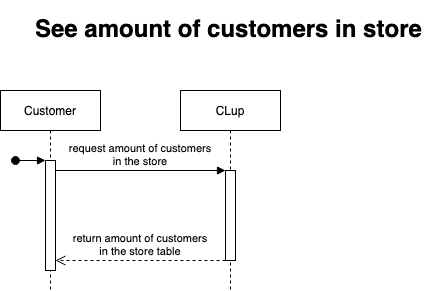
\includegraphics[height=0.5\textwidth]{Images/SequenceDiagrams/Customer/SeeAmountOfCustomersInStoreUseCaseSequenceDiagram.png}
    \caption{Sequence Diagram for Use Case: See amount of customers in the store}
\end{figure}

\begin{table}[H]
    \begin{tabular}{|p{8cm}|p{8cm}|}
        \hline
        \textit{Name}    & \textbf{See store location} \\ \hline
        \textit{Actors} & Customer, Maps API \\ \hline
        \textit{Entry conditions} & The customer needs to know where the store is located and the travel time \\ \hline
        % TODO: Are entry conditions things already met (user logged in) or intention (Customer wants, needs etc...)
        \textit{Event flows}      & \tabitem The customer clicks on the "Store Location" button. \\
        & \tabitem The application contacts the Maps API with the store location. \\
        & \tabitem The Maps API returns a map from the customer position to the store with a time estimation. \\
        \hline
        \textit{Exit conditions} & The customer knows how to go to the store and the travel time needed. \\ \hline
        \textit{Exceptions} & \tabitem The customer's smartphone doesn't provide or allow access to location services. \\
        \hline
    \end{tabular}
    \caption{Use Case: See store location}
\end{table}
\begin{figure}[H]
    \centering
    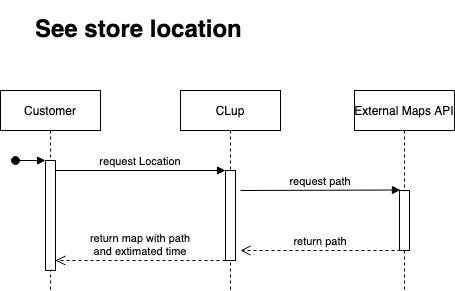
\includegraphics[height=0.5\textwidth]{Images/SequenceDiagrams/Customer/SeeStoreLocationUseCaseSequenceDiagram.png}
    \caption{Sequence Diagram for Use Case: See store location}
\end{figure}
\begin{table}[H]
    \begin{tabular}{|p{8cm}|p{8cm}|}
        \hline
        \textit{Name}    & \textbf{Sign up} \\ \hline
        \textit{Actors} & Customer \\ \hline
        \textit{Entry conditions} & The customer opened the application and they are not registered yet, and they want to register. \\ \hline
        \textit{Event flows}      & \tabitem The customer clicks on the "Sign Up" button. \\
        & \tabitem The customer inserts their credentials. \\
        & \tabitem The application sends the information to the server. \\
        & \tabitem The server stores the data related to the user. \\
        & \tabitem The server returns an acknowledgement to the app. \\
        \hline
        \textit{Exit conditions} & The customer is now registered and can use all the functionalities of the app. \\ \hline
        \textit{Exceptions} & \tabitem The e-mail provided in the registration form is already used by another user. \\
        & \tabitem The credentials provided in the registration form are ill-formatted.\\
        \hline
    \end{tabular}
    \caption{Use Case: Sign up}
\end{table}
\begin{figure}[H]
    \centering
    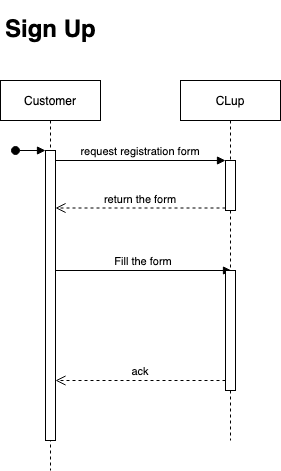
\includegraphics[height=0.5\textwidth]{Images/SequenceDiagrams/Customer/SignUpUseCaseSequenceDiagram.png}
    \caption{Sequence Diagram for Use Case: Sign up}
\end{figure}
\begin{table}[H]
    \begin{tabular}{|p{8cm}|p{8cm}|}
        \hline
        \textit{Name}    & \textbf{Login} \\ \hline
        \textit{Actors} & User \\ \hline
        \textit{Entry conditions} & The user has already sign up and wants to login to use CLup functionalities \\ \hline
        \textit{Event flows}     & \tabitem The customer clicks on the "Login" button\\
        & \tabitem The user provides their login credentials. \\
        & \tabitem The system authenticates the user \\
        \hline
        \textit{Exit conditions} & The user is logged in and can now use all the CLup functionalities \\ \hline
        \textit{Exceptions} & \tabitem The credentials are wrong \\
        \hline
    \end{tabular}
    \caption{Use Case: Login}
\end{table}
\begin{figure}[H]
    \centering
    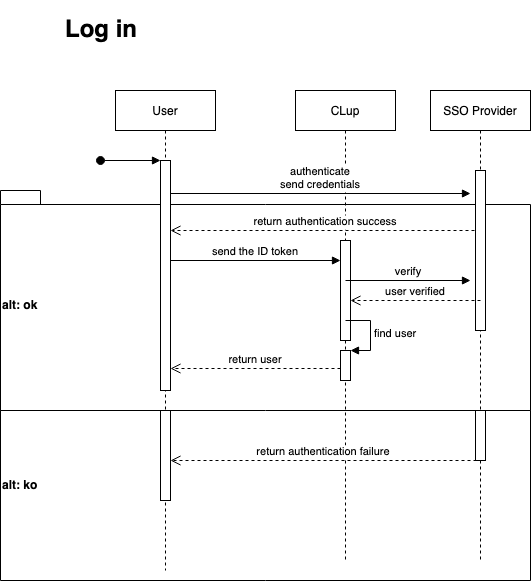
\includegraphics[height=0.5\textwidth]{Images/SequenceDiagrams/LogInUseCaseSequenceDiagram.png}
    \caption{Sequence Diagram for Use Case: Login}
\end{figure}
\begin{table}[H]
    \begin{tabular}{|p{8cm}|p{8cm}|}
        \hline
        \textit{Name}    & \textbf{Notify ticket delete} \\ \hline
        \textit{Actors} & Customer \\ \hline
        \textit{Entry conditions} & A ticket of the Customer was deleted from the server. \\ \hline
        \textit{Event flows}     & \tabitem The system sends an email to the customer to notify the deletion of their ticket\\
        \hline
        \textit{Exit conditions} & The customer is informed about the deletion of their ticket. \\ \hline
        \textit{Exceptions} & \tabitem \\
        \hline
    \end{tabular}
    \caption{Use Case: Notify ticket delete}
\end{table}
\begin{figure}[H]
    \centering
    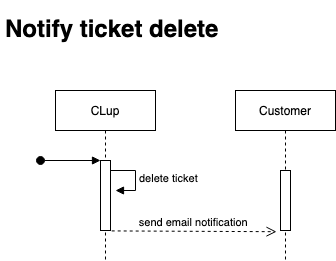
\includegraphics[height=0.5\textwidth]{Images/SequenceDiagrams/Customer/NotifyTicketDeleteUseCaseSequenceDiagram.png}
    \caption{Sequence Diagram for Use Case: Notify ticket delete}
\end{figure}
\begin{table}[H]
    \begin{tabular}{|p{8cm}|p{8cm}|}
        \hline
        \textit{Name}    & \textbf{Update user information} \\ \hline
        \textit{Actors} & User \\ \hline
        \textit{Entry conditions} & The user wants to change an information of themselves. \\ \hline
        \textit{Event flows}     & \tabitem The user clicks on the "Update User Information" button. \\
        & \tabitem The application shows a form precompiled with user's previous information. \\
        & \tabitem The user changes the information on the respective fields and presses the "Submit" button. \\
        & \tabitem The system saves the changes. \\
        \hline
        \textit{Exit conditions} & The user successfully updated their information. \\ \hline
        \textit{Exceptions} & \tabitem The new information provided is ill-formatted. \\
        \hline
    \end{tabular}
    \caption{Use Case: Update user information}
\end{table}
\begin{figure}[H]
    \centering
    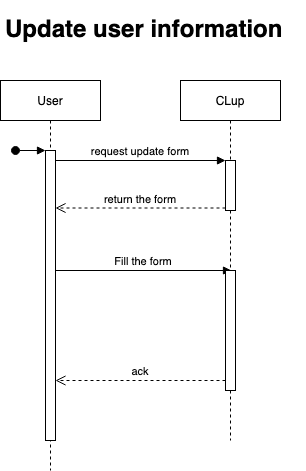
\includegraphics[height=0.5\textwidth]{Images/SequenceDiagrams/UpdateUserInformationUseCaseSequenceDiagram.png}
    \caption{Sequence Diagram for Use Case: Update user information}
\end{figure}


\begin{table}[H]
    \begin{tabular}{|p{8cm}|p{8cm}|}
        \hline
        \textit{Name}    & \textbf{Retrieve line number} \\ \hline
        \textit{Actors} & Customer \\ \hline
        \textit{Entry conditions} & The customer is logged in the application and wants to retrieve a line number. \\ \hline
        \textit{Event flows}      & \tabitem The customer clicks on the "retrieve line number" button in the application \\
        & \tabitem The application returns an ETA and ask confirm to the customer. \\
        & \tabitem The customer confirms. \\
        & \tabitem The customer ask the application to generate the QR code. \\
        & \tabitem The application returns the QR code. \\
        \hline
        \textit{Exit conditions} & The customer have retrieved a line number. \\ \hline
        \textit{Exceptions} & \tabitem The server cannot retrieve the line number since the time slot is full. \\ \hline
    \end{tabular}
    \caption{Use Case: Retrieve line number}
\end{table}
\begin{figure}[H]
    \centering
    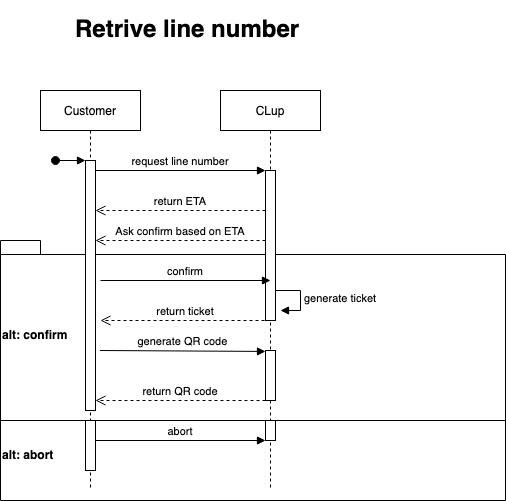
\includegraphics[height=0.5\textwidth]{Images/SequenceDiagrams/Customer/RetriveLineNumberUseCaseSequenceDiagram.png}
    \caption{Sequence Diagram for Use Case: Retrieve line number}
\end{figure}

\subsubsection{Clerk}

\begin{figure}[H]
    \centering
    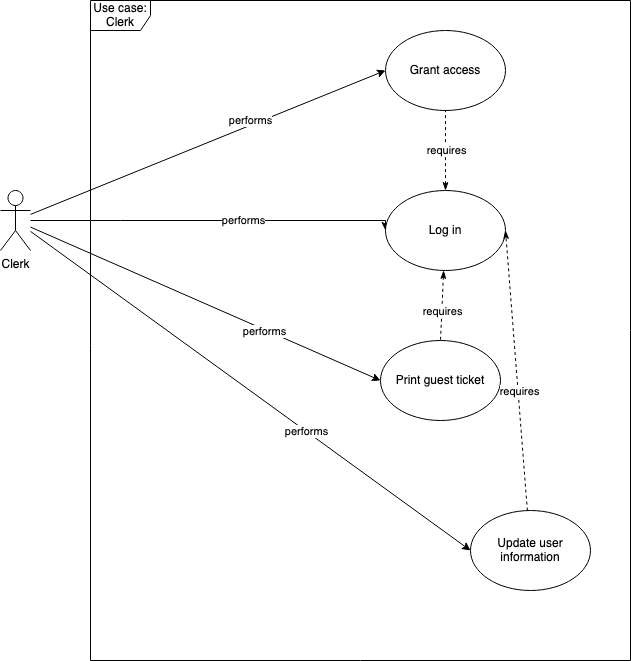
\includegraphics[height=0.5\textwidth]{Images/UseCaseDiagrams/Clerk.png}
    \caption{Use Case Diagram for Clerk}
\end{figure}

\textbf{Use cases}

\begin{table}[H]
    \begin{tabular}{|p{8cm}|p{8cm}|}
        \hline
        \textit{Name}    & \textbf{Grant access} \\ \hline
        \textit{Actors} & Clerk, Customer \\ \hline
        \textit{Entry conditions} & The customer has already obtained the QR code and they plan on entering the store.\\ \hline
        \textit{Event flows}      & \tabitem The Clerk scans the QR code from the customer's smartphone or printed ticket using the application \\
        & \tabitem The application analyzes the QR code and contacts to the Server \\
        & \tabitem The server decides if the customer can enter based on the information received in the QR code \\
        & \tabitem The server responds to the clerk application with the result \\
        & \tabitem The clerk let the customer enter the store \\ % TODO: Are we supposed to write about world phenomena?
        \\ \hline
        \textit{Exit conditions} & The customer enters the store \\ \hline
        \textit{Exceptions} & \tabitem The server communicates to the clerk that the customer cannot enter because their line number is not available.\\ \hline
    \end{tabular}
    \caption{Use Case: Grant access}
\end{table}
\begin{figure}[H]
    \centering
    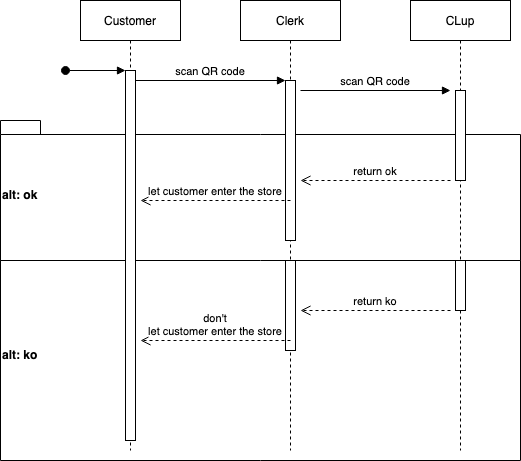
\includegraphics[height=0.5\textwidth]{Images/SequenceDiagrams/Clerk/GrantAccessUseCaseSequenceDiagram.png}
    \caption{Sequence Diagram for Use Case: Grant Access}
\end{figure}
\begin{table}[H]
    \begin{tabular}{|p{8cm}|p{8cm}|}
        \hline
        \textit{Name}    & \textbf{Print guest ticket} \\ \hline
        \textit{Actors} & Clerk, Customer \\ \hline
        \textit{Entry conditions} & The customer has arrived to the location, doesn't have a ticket on their smartphone, and needs a physical ticket to enter. \\ \hline
        \textit{Event flows}      & \tabitem The customer asks the clerk for a ticket. \\
        & \tabitem The clerk generate a ticket using the app. \\
        & \tabitem The application sends a request to the server to generate a ticket. \\
        & \tabitem The server generates a line number and a ticket. \\
        & \tabitem The server sends the ticket back to the app. \\
        & \tabitem The clerk prints the ticket. \\ % TODO: Real world phenomena here again?
        & \tabitem The clerk gives the ticket to the customer. \\
        \hline
        \textit{Exit conditions} & The customer has a ticket. \\ \hline
        \textit{Exceptions} & \tabitem The server cannot generate a line number due to capacity constraints. \\ \hline
    \end{tabular}
    \caption{Use Case: Print guest ticket}
\end{table}
\begin{figure}[H]
    \centering
    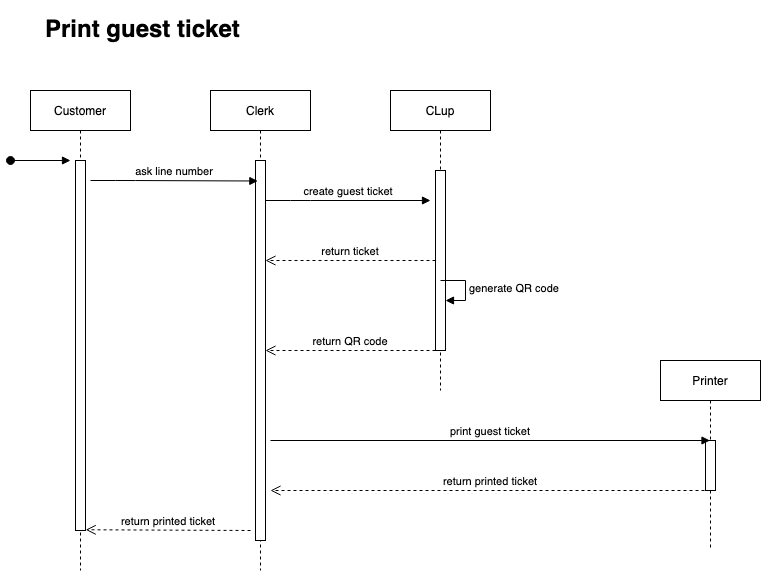
\includegraphics[height=0.5\textwidth]{Images/SequenceDiagrams/Clerk/PrintGuestTicketUseCaseSequenceDiagram.png}
    \caption{Sequence Diagram for Use Case: Print guest ticket}
\end{figure}


\subsubsection{Manager}

\begin{figure}[H]
    \centering
    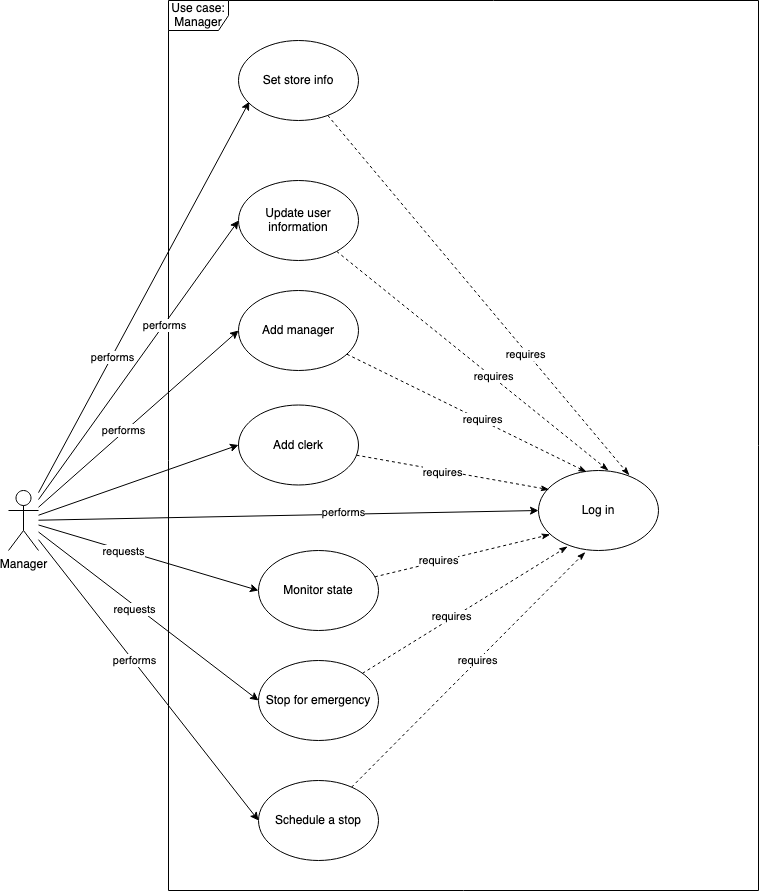
\includegraphics[height=0.5\textwidth]{Images/UseCaseDiagrams/Manager.png}
    \caption{Use Case Diagram for Manager}
\end{figure}

\textbf{Use cases}

\begin{table}[H]
    \begin{tabular}{|p{8cm}|p{8cm}|}
        \hline
        \textit{Name}    & \textbf{Initialize} \\ \hline
        \textit{Actors} & Manager \\ \hline
        \textit{Entry conditions} & The manager of the store needs to set the basic information of the store in order to start the service \\ \hline
        \textit{Event flows}      & \tabitem The manager clicks on the initialize button \\
        & \tabitem The application shows the location form to the manager \\
        & \tabitem The manager fills the form and sends ıt to the server via the app\\
        & \tabitem The server registers the information and acknowledges \\
        \hline
        \textit{Exit conditions} & The system is initialized and can offer all its functions \\ \hline
        \textit{Exceptions} & \tabitem Some mandatory parts of the form are not filled. \\ \hline
    \end{tabular}
    \caption{Use Case: Initialize}
\end{table}

% TODO: There is no request for info form, front-end is capable of generating such info.
\begin{figure}[!htbp]
    \centering
    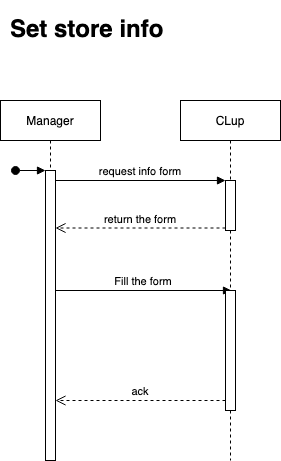
\includegraphics[height=0.5\textwidth]{Images/SequenceDiagrams/Manager/SetStoreInfoUseCaseSequenceDiagram.png}
    \caption{Sequence Diagram for Use Case: Initialize}
\end{figure}
\begin{table}[H]
    \begin{tabular}{|p{8cm}|p{8cm}|}
        \hline
        \textit{Name}    & \textbf{Monitor state} \\ \hline
        \textit{Actors} & Manager \\ \hline
        \textit{Entry conditions} & The manager wants to monitor the number of customers in the store in real time. \\ \hline
        \textit{Event flows}      & \tabitem The manager clicks on the "Monitoring" button. \\
        & \tabitem The application sends the number request to the server.  \\
        & \tabitem The server returns the number of customers in the store. \\
        & \tabitem The application repeats the process periodically as long as the monitoring page is open. \\ % TODO: What period? Do we need to specify this?
        \hline
        \textit{Exit conditions} & The manager is informed on the number of the customers in the store in real time. \\ \hline
        \textit{Exceptions} & \tabitem \\ \hline
    \end{tabular}
    \caption{Use Case: Monitor state}
\end{table}
\begin{figure}[H]
    \centering
    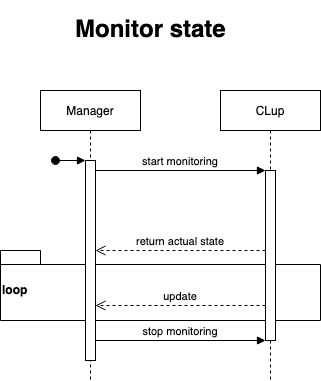
\includegraphics[height=0.5\textwidth]{Images/SequenceDiagrams/Manager/MonitorStateUseCaseSequenceDiagram.png}
    \caption{Sequence Diagram for Use Case: Monitor state}
\end{figure}
\begin{table}[H]
    \begin{tabular}{|p{8cm}|p{8cm}|}
        \hline
        \textit{Name}    & \textbf{Schedule a stop} \\ \hline
        \textit{Actors} & Manager \\ \hline
        \textit{Entry conditions} & The manager wants to schedule a period of time in which the store will be closed so the users can not book a visit for that time. \\ \hline
        \textit{Event flows}      & \tabitem The manager clicks on the "Schedule a Stop" button. \\
        & \tabitem The application shows a form for the time of the stop. \\
        & \tabitem The manager fills the form and submits it to the server through the app. \\
        & \tabitem The server stores the information in the database and returns an acknowledgement. \\
        \hline
        \textit{Exit conditions} & The system has a scheduled stop stored in its database and will use it to prevent customers from booking a visit in that time period. \\ \hline
        \textit{Exceptions} & \tabitem There is already a planned stop in that period. \\ \hline
    \end{tabular}
    \caption{Use Case: Schedule a stop}
\end{table}
\begin{figure}[H]
    \centering
    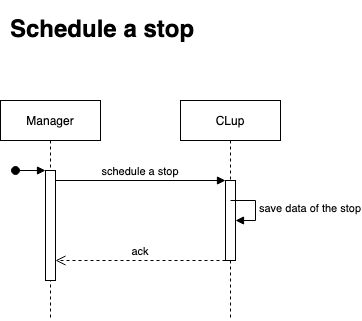
\includegraphics[height=0.5\textwidth]{Images/SequenceDiagrams/Manager/ScheduleAStopUseCaseSequenceDiagram.png}
    \caption{Sequence Diagram for Use Case: Schedule a stop}
\end{figure}
\begin{table}[H]
    \begin{tabular}{|p{8cm}|p{8cm}|}
        \hline
        \textit{Name}    & \textbf{Stop for emergency} \\ \hline
        \textit{Actors} & Manager \\ \hline
        \textit{Entry conditions} & An emergency occurred and the manager wants to immediately stop the system from distributing line numbers. \\ \hline
        \textit{Event flows}     & \tabitem The manager click on the "Emergency Stop" button \\
        & \tabitem The application asks for confirmation from the manager. \\
        & \tabitem The manager confirms the stop of the system. \\
        & \tabitem The application sends the system stop request to the server. \\
        & \tabitem The server stops the service and return an acknowledgement. \\
        \hline
        \textit{Exit conditions} & The system has interrupted the service. \\ \hline
        \textit{Exceptions} & \tabitem The manager aborts the operation. \\
        \hline
    \end{tabular}
    \caption{Use Case: Stop for emergency}
\end{table}
\begin{figure}[H]
    \centering
    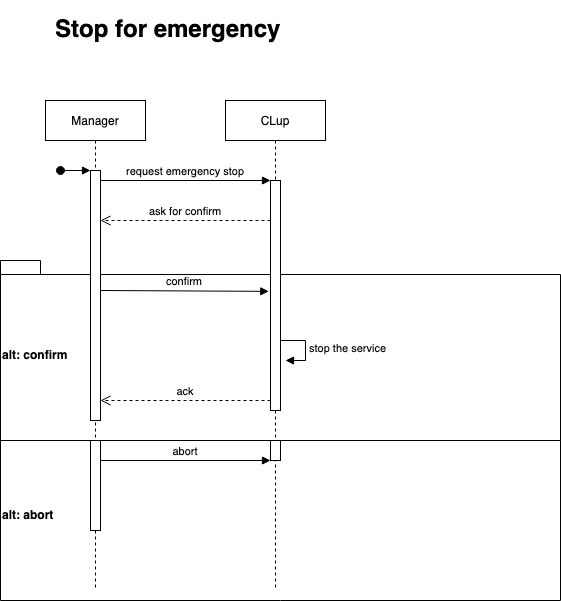
\includegraphics[height=0.5\textwidth]{Images/SequenceDiagrams/Manager/StopForEmergencyUseCaseSequenceDiagram.png}
    \caption{Sequence Diagram for Use Case: Stop for emergency}
\end{figure}
\begin{table}[H]
    \begin{tabular}{|p{8cm}|p{8cm}|}
        \hline
        \textit{Name}    & \textbf{Add Clerk} \\ \hline
        \textit{Actors} & Manager \\ \hline
        \textit{Entry conditions} & The manager wants to add a new clerk to the system \\ \hline
        \textit{Event flows}     & \tabitem The manager click on the "add clerk" button \\
        & \tabitem The system asks the data of the new clerk (e.g. the credentials) \\
        & \tabitem The manager inserts the data and press "submit" \\
        \hline
        \textit{Exit conditions} & The new clerk is added to the system \\ \hline
        \textit{Exceptions} & \tabitem The data of the clerk are incomplete or incorrect \\
        \hline
    \end{tabular}
    \caption{Use Case: Add Clerk}
\end{table}
\begin{figure}[H]
    \centering
    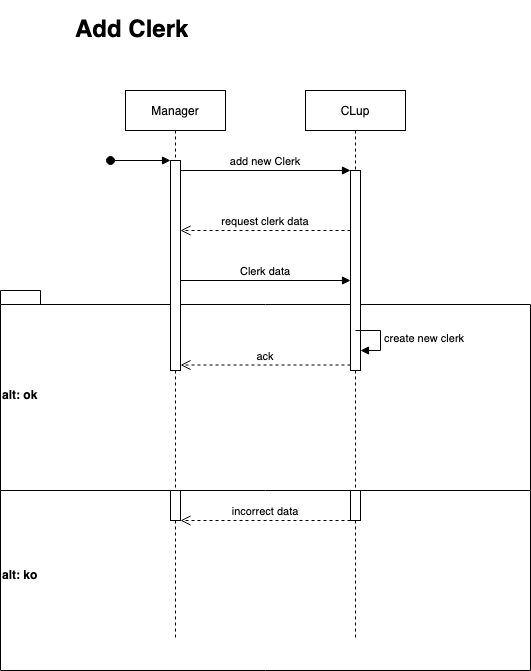
\includegraphics[height=0.5\textwidth]{Images/SequenceDiagrams/Manager/AddClerkUseCaseSequenceDiagram.png}
    \caption{Sequence Diagram for Use Case: Add Clerk}
\end{figure}
\begin{table}[H]
    \begin{tabular}{|p{8cm}|p{8cm}|}
        \hline
        \textit{Name}    & \textbf{Add Manager} \\ \hline
        \textit{Actors} & Manager \\ \hline
        \textit{Entry conditions} & The manager wants to add a new manager to the system \\ \hline
        \textit{Event flows}     & \tabitem The manager click on the "Add Manager" button \\
        & \tabitem The system asks the data of the new manager (e.g. the credentials) \\
        & \tabitem The manager inserts the data and press "Submit" \\
        \hline
        \textit{Exit conditions} & The new Manager is added to the system \\ \hline
        \textit{Exceptions} & \tabitem The data of the Manager are incomplete or incorrect \\
        \hline
    \end{tabular}
    \caption{Use Case: Add Manager}
\end{table}
\begin{figure}[H]
    \centering
    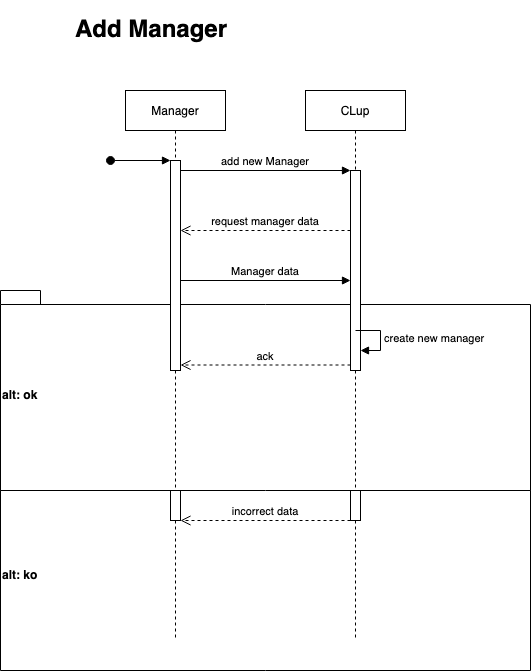
\includegraphics[height=0.5\textwidth]{Images/SequenceDiagrams/Manager/AddManagerUseCaseSequenceDiagram.png}
    \caption{Sequence Diagram for Use Case: Add Manager}
\end{figure}

\subsubsection{Requirements}
\begin{itemize}
    \item \textbf{$R_{1}$} The system must allow users to authenticate using their e-mail address and password.
    \item \textbf{$R_{2}$} The system must allow customers to register using their e-mail address, their name, surname, phone number, and a new password.
    \item \textbf{$R_{3}$} Managers must be able to add additional managers and clerks as users.
    \item \textbf{$R_{4}$} Managers must be able to set and update location-specific information, that is, the maximum number of customers in the location at any given time, opening and closing hours of the store per each day, line number timeout, the limit of reservation per customer on a predetermined time interval that is one of the month, week or day, and location of the place % One form
    \item \textbf{$R_{5}$} Managers can add any other location as a partner store.
    \item \textbf{$R_{6}$} Managers can stop the system from issuing any more tickets for a given day
    \item \textbf{$R_{7}$} Managers can schedule the system stop for a future time.
    \item \textbf{$R_{8}$} Managers can set the in-shop locations for different categories and product items.
    \item \textbf{$R_{9}$} In case of a system stop, no further line numbers can be issued for the given time slots.
    \item \textbf{$R_{10}$} In case of a system stop, all line numbers in the stop time slots has to be canceled.
    \item \textbf{$R_{11}$} The system must cancel those line numbers that the customer did not arrive at the location for more than the set timeout interval.
    \item \textbf{$R_{12}$} In case of ticket cancellation, the customer must be notified with an e-mail notification.
    \item \textbf{$R_{13}$} Clerks must register the entrance and exit of customers via scanning the QR code for their line number.
    \item \textbf{$R_{14}$} Clerks must be able to generate line number tickets in a compatible printer format.
    \item \textbf{$R_{15}$} Customers must be able to obtain a line number, except when the system is stopped, or the store is full.
    \item \textbf{$R_{16}$} Customers must be able to obtain line numbers for different time slots in the future.
    \item \textbf{$R_{17}$} Customers can not obtain line numbers that exceed the quantity per time interval limits.
    \item \textbf{$R_{18}$} Customers can not obtain line numbers for time intervals that the system is stopped by a manager.
    \item \textbf{$R_{19}$} Customers must be able to see the estimated time available for their line number.
    \item \textbf{$R_{20}$} Customers must be able to set or update their phone number, password, name, and surname.
    \item \textbf{$R_{21}$} Customers can select a specific product or product categories they plan to visit in the location while obtaining a line number.
    \item \textbf{$R_{22}$} Customers can set an estimated time for their visit while obtaining a line number.
    \item \textbf{$R_{23}$} Customers must be able to view the shop location
    \item \textbf{$R_{24}$} Customers can view the occupation forecasts for the location at different time slots.
    \item \textbf{$R_{25}$} Customers can see the alternative suggestions for time slots while obtaining a line number for the future.
    \item \textbf{$R_{26}$} Customers can view the occupancy for the partner stores if the preferred time slot is not available while obtaining a line number.
    \item \textbf{$R_{27}$} The system must be able to provide a forecast for each location's occupancy for any given time based on past visits.
\end{itemize}


% Goals, mapped to the requirements and domain assumptions they relate to
% (Requirements are vaguely given in Overview -> Product functions)
% (Domain assumptions are in Overview -> Assumptions,dependencies and constraints -> Domain Assumptions)
\subsubsection{Summary Table}
\begin{table}[H]
    \begin{tabular}{|p{1cm}|p{7cm}|p{7cm}|}
        \hline
        \textbf{Goal} & \textbf{Requirements} & \textbf{Domain Assumptions} \\ \hline
        $G_{1}$ & $R_{1}$, $R_{2}$, $R_{11}$, $R_{15}$, $R_{17}$, $R_{18}$ & $D_{1}$, $D_{13}$\\ \hline
        $G_{2}$ & $R_{1}$, $R_{2}$, $R_{11}$, $R_{16}$, $R_{17}$, $R_{18}$, $R_{26}$ & $D_{1}$\\ \hline
        $G_{3}$ & $R_{1}$, $R_{2}$, $R_{8}$, $R_{21}$, $R_{22}$ & $D_{1}$\\ \hline
        $G_{4}$ & $R_{1}$, $R_{2}$, $R_{12}$, $R_{19}$, $R_{23}$, $R_{24}$, $R_{27}$ & $D_{1}$, $D_{3}$, $D_{6}$, $D_{8}$\\ \hline
        $G_{5}$ & $R_{1}$, $R_{2}$, $R_{5}$, $R_{24}$, $R_{25}$, $R_{26}$ & $D_{1}$\\ \hline
        $G_{6}$ & $R_{1}$, $R_{3}$, $R_{6}$, $R_{7}$, $R_{9}$, $R_{10}$, $R_{12}$, $R_{18}$ & $D_{1}$, $D_{11}$\\ \hline
        $G_{7}$ & $R_{1}$, $R_{3}$, $R_{4}$, $R_{11}$, $R_{17}$, $R_{27}$ & $D_{1}$, $D_{7}$\\ \hline
        $G_{8}$ & $R_{1}$, $R_{3}$, $R_{13}$, $R_{20}$ & $D_{1}$, $D_{3}$, $D_{4}$, $D_{5}$, $D_{6}$, $D_{9}$, $D_{11}$, $D_{12}$, $D_{13}$\\ \hline
        $G_{9}$ & $R_{3}$, $R_{14}$ & $D_{2}$, $D_{6}$, $D_{10}$, $D_{13}$\\ \hline
    \end{tabular}
    \caption{Summary Table}
\end{table}

\iffalse
Usecases:
Customer:

Book future line number
See amount of customers in the store
See store location
Sign Up
Login
Notify ticket delete
Update user information
Retrieve line number

Clerk:
Grant access
Print Guest Ticket

Manager:
Initialize
Monitor State
Schedule a stop
Stop for Emengency
Add clerk
Add manager
\fi
\subsubsection{Tracability Matrix}
\begin{table}[H]
    \begin{tabular}{|p{8cm}|p{8cm}|}
        \hline
        \textbf{Requirement} & \textbf{Use case} \\ \hline
        $R_{1}$ & Login\\ \hline
        $R_{2}$ & Sign Up\\ \hline
        $R_{3}$ & Add Clerk\\
        & Add Manager \\ \hline
        $R_{4}$ & Initialize \\ \hline
        $R_{5}$ & Initialize \\ \hline
        $R_{6}$ & Stop for Emergency\\ \hline
        $R_{7}$ & Schedule a Stop\\ \hline
        $R_{8}$ & Initialize \\ \hline
        $R_{9}$ & Schedule a Stop\\
        & Stop for Emergency \\ \hline
        $R_{10}$ & Schedule a Stop\\
        & Stop for Emergency\\ \hline
        $R_{11}$ & Retrieve Line Number\\ \hline
        $R_{12}$ & Notify Ticket Delete \\ \hline
        $R_{13}$ & Grant Access \\ \hline
        $R_{14}$ & Print Guest Ticket \\ \hline
        $R_{15}$ & Retrieve Line Number \\ \hline
        $R_{16}$ & Book Future Line Number\\ \hline
        $R_{17}$ & Book Future Line Number\\
        & Initialize \\ \hline
        $R_{18}$ & Book Future Line Number \\
        & Schedule a Stop \\
        & Stop for Emergency\\ \hline
        $R_{19}$ & Retrieve Line Number \\ \hline
        $R_{20}$ & Update User Information\\ \hline
        $R_{21}$ & Book Future Line Number\\ \hline
        $R_{22}$ & Book Future Line Number\\ \hline
        $R_{23}$ & See Store Location\\ \hline
        $R_{24}$ & See Amount of Customers in the Store\\ \hline
        $R_{25}$ & Book Future Line Number\\ \hline
        $R_{26}$ & Book Future Line Number\\ \hline
        $R_{27}$ & See Number of Customers in the Store\\ \hline
    \end{tabular}
    \caption{Tracability Matrix}
\end{table}
\subsection{Performance Requirements}

% Some basic stuff about how much users the system takes, speed etc...

% TODO: @Hrvoje Complete these
\subsection{Design Constraints}
%Specify constraints on the system design imposed by external standards, regulatory requirements, or project limitations.

\subsubsection{Standards compliance}
% QR standard, UTC timing standard, GPS, etc...

%Specify the requirements derived from existing standards or regulations, including:
%a) Report format;
%b) Data naming;
%c) Accounting procedures;
%d) Audit tracing.
%For example, this could specify the requirement for software to trace processing activity.
%Such traces are needed for some applications to meet minimum regulatory or financial standards.
%An audit trace requirement may, for example, state that all changes to a payroll database shall be recorded in a trace file with before and after values.

The code produced should follow the requirements contained in this document. Furthermore, its comments should be clear and focused. The application will use QR code generated accordingly with the ISO/IEC 18004:2015 standard. All date and time shown will be in compliance with the ISO 8601 UTC timing standard.

\subsubsection{Hardware limitations}
% What needs to be on the phone?

To be able to use the application, customer should have a smartphone, tablet or desktop computer with working display, input device such as keyboard, physical or on touch screen keyboard and active internet connection. Clerk should have smartphone with working display, input device and a working camera module and active internet connection. Manager should have a desktop computer with working display, input device and active internet connection.

\subsubsection{Any other constraint}
% GDPR regulations, local laws, etc...

% Isn't this similar to Overview -> Assumptions,dependencies and constraints -> Constraints?
% Everything is similar to everything

The application will use and store users data accordingly with GDPR rules.

\subsection{Software System Attributes}

\subsubsection{Reliability}
% Don't crash for long time, fault tolerance strategies like RAID, backups, etc

% Specify the factors required to establish the required reliability of the software system at time of delivery.

The application should produce the same results independet on the system it is used on. For example, a customer should be able to schedule a time visit for a store using either his smartphone, tablet or desktop computer. The application should give consistently correct results.

\subsubsection{Availability}
% 99.5% availability minimum, release any hardware control in case of power cut or unavailability.

% Specify the factors required to guarantee a defined availability level for the entire system such as checkpoint, recovery, and restart.

The system should have 99,5\% available time per month with maximum monthly 33m 49.7s downtime. In case of upgrade or maintenance, the maintenance window will be out of business hours.

\subsubsection{Security}
% Data hashing, salting, encryption of user data if necessary.

% Specify the requirements to protect the software from accidental or malicious access, use modification, destruction, or disclosure.

System integrity or security should be sufficient to prevent unauthorized access to application functions, preventing information loss, ensure that the application is protected from virus infection, and protecting the privacy of data entered into the system. All user data must be encrypted before being stored. Furthermore all passwords must be hashed.

\subsubsection{Maintainability}
% Testing practices on all levels

% Specify attributes of software that relate to the ease of maintenance of the software itself. These may include requirements for certain modularity, interfaces, or complexity limitation.

Application should be developed before the Covid-19 crises ends. Its maintainability isn't concern since the application will be developed for the purpose of this pandemic only.

\subsubsection{Portability}
% Usage of widely adopted platforms (Java, .NET, Browser), no custom protocol implementation apart from wide-spread

% Specify attributes of software that relate to the ease of porting the software to other host machines and/or operating systems, including:

Application should be available to vast majority of people.
